\documentclass{standalone} 
\usepackage{tikz}
\usetikzlibrary{external}
\usetikzlibrary{trees}
\usetikzlibrary{arrows}
\begin{document}
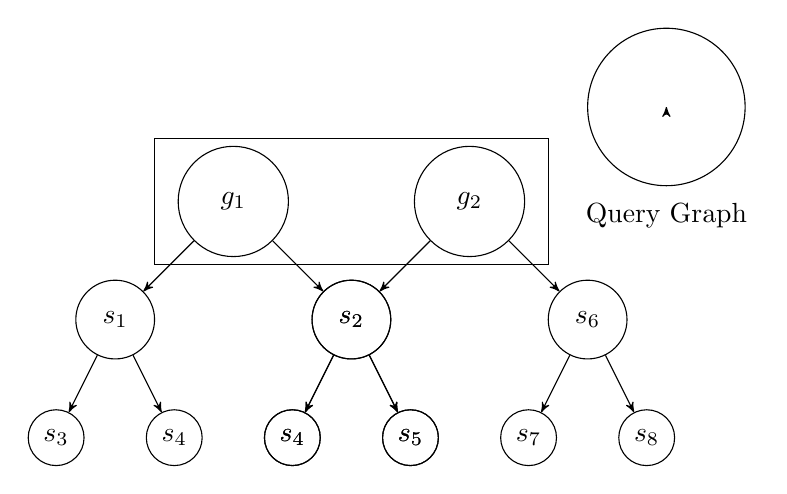
\begin{tikzpicture}[scale=1.0,level distance=1.5cm,
  level 1/.style={sibling distance=3cm},
  level 2/.style={sibling distance=1.5cm},
  level 3/.style={sibling distance=1.5cm},
  -stealth',
  every node/.style={circle, draw=black,thin, minimum size = 0.5cm},
  no_edge/.style={edge from parent/.style={red,very thick,draw}},
  norm_edge/.style={edge from parent/.style={black,thin,draw}},
  l1_node_size/.style={circle, draw=black,thin, minimum size = 1.4cm},
  l2_node_size/.style={circle, draw=black,thin, minimum size = 1.0cm},
  l3_node_size/.style={circle, draw=black,thin, minimum size = 0.5cm},
  every edge/.style={path=[->], draw=black,thin, minimum}]
%  \draw[help lines] (-5,-6) grid (10,6);
  \begin{scope}[shift={(-2,0)}]
  \node[l1_node_size] {$g_1$}
  	child {node[l2_node_size] {$s_1$}
      	child {node[l3_node_size] {$s_3$}}
      	child {node[l3_node_size] {$s_4$}}
      	}
    child {node[l2_node_size] {$s_2$}
      	child {node[l3_node_size] {$s_4$}}
      	child {node[l3_node_size] {$s_5$}}
      	}
    ;
    \end{scope}
  \begin{scope}[shift={(1,0)}]
  \node[l1_node_size] {$g_2$}
  	child {node[l2_node_size] {$s_2$}
      	child {node[l3_node_size] {$s_4$}}
      	child {node[l3_node_size] {$s_5$}}
      	}
    child {node[l2_node_size] {$s_6$}
      	child {node[l3_node_size] {$s_7$}}
      	child {node[l3_node_size] {$s_8$}}
      	}
    ;
    \end{scope}
    \begin{scope}[shift={(-2,0)}]
 	   \draw (-1,-.8) rectangle (4,.8);
% 	   \path[draw] (-1,-.8) node[rectangle,minimum size=(5.0cm,1.0cm),label={[yshift=0.8cm]above:Graph Database}]{}
    \end{scope}
\begin{scope}[shift={(2.5,0.2)}]
	\draw (1,1) node[circle,minimum size = 2.0cm,label={[yshift=0.8cm]below:Query Graph}]{};
\end{scope}
\end{tikzpicture}
\end{document}